Projekt miał na celu utworzenie kompletnego systemu przetwarzania danych wektorowych, składającego się z trzech głównych części:

\begin{itemize}
  \item dedykowanego, wysokopoziomowego języka programowania, stworzonego z myślą o danych wektorowych,
  \item procesora zaimplementowanego na układzie FPGA, uwzględniającego w swojej architekturze ukierunkowanie na przetwarzanie wektorów,
  \item modułu pozwalającego na komunikację między dwiema powyższymi częściami.
\end{itemize}

\begin{figure}
  \begin{center}
    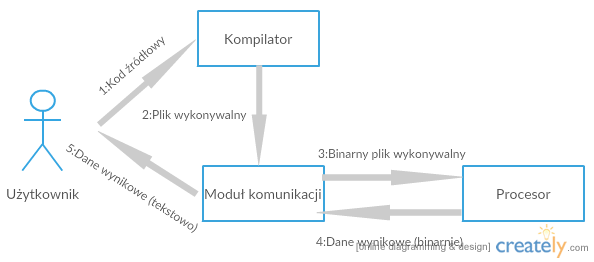
\includegraphics[scale=0.5]{images/SystemOverview.png}
    \caption{Schemat działania systemu. Na diagramie przedstawiono główne komponenty systemu i ich współdziałanie.}
    \label{fig:file-structure}
  \end{center}
\end{figure}

W niniejszej dokumentacji znajduje się opis modułów, z których składa się każda z części wraz ze sposobem ich funkcjonowania oraz niektórymi przesłankami stojącymi za sposobem ich implementacji (wybrana technologia stworzenia kompilatora --- język Haskell i jego ekosystem --- jest na tyle niecodzienna, że staramy się przedstawić czytelnikowi jej wyjątkowo dobre przystosowanie do tworzenia kompilatorów i podobnego oprogramowania).

\section{Struktura projektu}

Struktura projektu, a wraz z nią struktura repozytorium, odzwierciedla wyraźny podział na część software'ową (kompilator naszego języka programowania) oraz hardware'ową (koprocesor zaimplementowany na układzie FPGA). Dodatkowo, dokumentacja do projektu jest również trzymana w repozytorium, co umożliwia łatwiejszą współpracę nad jej tworzeniem i pozwala na zarządzanie jej wersjami.

Część hardware'owa, związana z FPGA, ma niemalże płaską strukturę: mamy jeden moduł główny i kilka pomniejszych komponentów, które są do niego dołączone (jako osobne części układu zaimplementowane są jego wyróżnione składowe, takie jak stos, pamięć ram czy moduł UART). Każdy z komponentów umieszczony jest w oddzielnym pliku.

Część software'owa jest w pełni autonomicznym projektem języka Haskell, budowanym systemem budowania Cabal. Narzuca to pewną strukturę plików i katalogów (w Haskellu tworzone są hierarchiczne moduły poprzez umieszczanie plików w odpowiednich ścieżkach folderów). Projekt podzielony jest na części związane z etapami kompilacji programów w naszym języku, w szczególności na dwa główne moduły: \texttt{Parser} i \texttt{CodeGen}, które z kolei podzielone są na bardziej szczegółowe submoduły. Dokładna struktura plików i katalogów została przedstawiona na rysunku \ref{fig:file-structure}.

\begin{figure}
  \begin{center}
    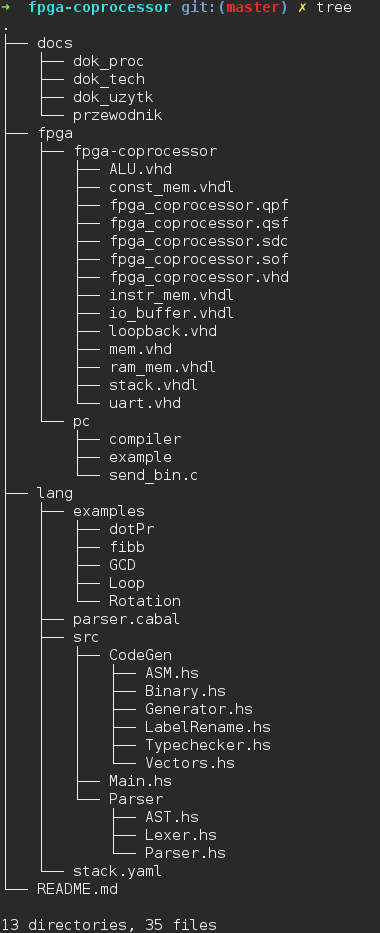
\includegraphics[scale=0.5]{images/file_structure.png}
    \caption{Struktura plików w projekcie jako wynik polecenia \texttt{tree} w systemie Linux.}
    \label{fig:file-structure}
  \end{center}
\end{figure}
